\chapter{开发周期}


    \section{合作方法}

        \subsection{开发环境}
        % Leap Motion官方Python2 SDK, 具体的环境说明以及配置方法见Git仓库的README。
        % TODO:The repo is private... although TA may never visit it.
        项目使用Leap Motion官方Python2 SDK进行开发,代码托管在GitHub仓库上\footnote{https://github.com/yuhui-zh15/AirGuitar}。

            \paragraph{后端开发环境} 后端开发环境主要指使用Leap Motion Python SDK实现的事件处理后台。

            % TODO:although failed to make it work on Windows T^T
            以下所有工具均可在Windows、Mac OS、Linux中的任意一个平台上运行,实现了跨平台开发。

            \tablethreeL{工具}{版本号}{简要说明}
                Leap Motion Python2 SDK & 2.3.1 & 用于感知用户双手的运动并转化为事件帧 \\
                fluidsynth & 依具体平台而不同 & 音乐库,包含各种MIDI中典型乐器的音色 \\
                mingus & 0.5.1 & Python音乐库模块,用于编程调用 \\
                flask & 0.12.2 & Python Web框架,用于和前端通信 \\
                flask-cors & 3.0.3 & 用于在flask框架上实现跨域资源共享(CORS) \\
            \tableend

            \paragraph{前端开发环境} 前端开发环境主要指基于HTML+CSS+JavaScript开发的用户界面。

            \tablethreeL{工具}{版本号}{简要说明}
                jQuery & 1.11.0 & 用于简化JavaScript代码结构 \\
            \tableend

            \paragraph{文档工具} 文档工具用于为项目构建清晰的接口说明文档。
            \tablethreeL{工具}{版本号}{简要说明}
                sphinx & 1.6.5 & 文档生成工具 \\
                sphinx-rtd-theme & 0.2.4 & 文档主题库 \\
            \tableend

        \subsection{设计模式}
            \paragraph{观察者模式(Observer)}
            ChordHandler, StrummingHandler分别处理Leap motion到来的帧,分开左手与右手的处理,并且不用修改主程序。

            \paragraph{组合(Aggregation)} 一个吉他模拟器Guitar实例将提供set\_chord, play\_string方法,使\
            处理输入数据后可以方便地改变吉他的状态。

    \section{迭代开发}

        \subsection{开发计划}
        以下给出AirGuitar的迭代开发计划:

            \paragraph{Sprint 1} 环境配置、初步实现左右手交互功能。
            \begin{enumerate}
                \itembf{音乐库}:选择并配置Python跨平台音乐库。
                \itembf{右手扫弦初步实现}:初步实现右手扫动时发出乐音的功能。
                \itembf{左手选择和弦初步实现}:初步实现九宫格式选择和弦功能,并留好接口以备扩展。
            \end{enumerate}

            \paragraph{Sprint 2} 功能完善、UI制作。
            \begin{enumerate}
                \itembf{右手扫弦功能完善}:通过高度限制,增强右手扫弦防误触功能。
                \itembf{左手选择和弦完善}:增加左手和弦识别功能。
                \itembf{UI}:基于Web框架实现UI,为后台准备接口。
            \end{enumerate}

            \paragraph{Sprint 3} 连接前后端、精度提升。
            \begin{enumerate}
                \itembf{前后端通信}:通过轮询方式实现后台和前端UI的数据通信。
                \itembf{左手选择和弦精度提升}:通过在UI增加反馈机制、视觉线索等,提高左手选择和弦的精度。
            \end{enumerate}

            \paragraph{Sprint 4} 用户实验、完成文档。
            \begin{enumerate}
                \itembf{用户实验}:收集学习时间、操作准确度等数据。
                \itembf{开发文档}:进行项目总结,完成文档。
            \end{enumerate}

        \subsection{版本控制}
        使用Git作为版本控制和分支管理的工具,任务分配通过GitHub上的Issue功能开展。

        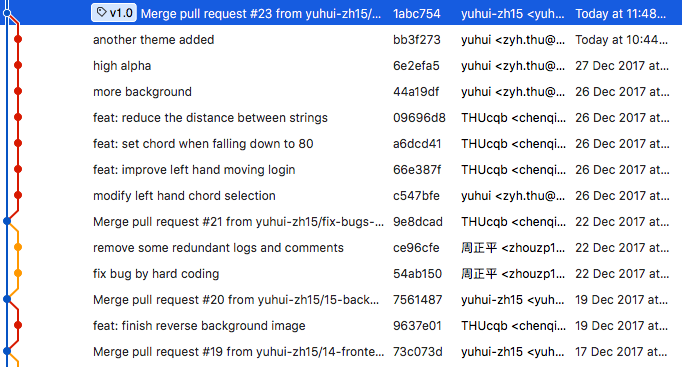
\includegraphics[width=\textwidth]{git}

        \subsection{项目管理}
        Merge Request组员都会收到并且互相进行Code Review,使我们代码质量较高、\
        开发进度也一直较快,在阶段展示的时候完成度就已经非常高。

        由于设备只有一台,故大多数时候其实并不能并行开发。
